\documentclass[1p]{elsarticle_modified}
%\bibliographystyle{elsarticle-num}

%\usepackage[colorlinks]{hyperref}
%\usepackage{abbrmath_seonhwa} %\Abb, \Ascr, \Acal ,\Abf, \Afrak
\usepackage{amsfonts}
\usepackage{amssymb}
\usepackage{amsmath}
\usepackage{amsthm}
\usepackage{scalefnt}
\usepackage{amsbsy}
\usepackage{kotex}
\usepackage{caption}
\usepackage{subfig}
\usepackage{color}
\usepackage{graphicx}
\usepackage{xcolor} %% white, black, red, green, blue, cyan, magenta, yellow
\usepackage{float}
\usepackage{setspace}
\usepackage{hyperref}

\usepackage{tikz}
\usetikzlibrary{arrows}

\usepackage{multirow}
\usepackage{array} % fixed length table
\usepackage{hhline}

%%%%%%%%%%%%%%%%%%%%%
\makeatletter
\renewcommand*\env@matrix[1][\arraystretch]{%
	\edef\arraystretch{#1}%
	\hskip -\arraycolsep
	\let\@ifnextchar\new@ifnextchar
	\array{*\c@MaxMatrixCols c}}
\makeatother %https://tex.stackexchange.com/questions/14071/how-can-i-increase-the-line-spacing-in-a-matrix
%%%%%%%%%%%%%%%

\usepackage[normalem]{ulem}

\newcommand{\msout}[1]{\ifmmode\text{\sout{\ensuremath{#1}}}\else\sout{#1}\fi}
%SOURCE: \msout is \stkout macro in https://tex.stackexchange.com/questions/20609/strikeout-in-math-mode

\newcommand{\cancel}[1]{
	\ifmmode
	{\color{red}\msout{#1}}
	\else
	{\color{red}\sout{#1}}
	\fi
}

\newcommand{\add}[1]{
	{\color{blue}\uwave{#1}}
}

\newcommand{\replace}[2]{
	\ifmmode
	{\color{red}\msout{#1}}{\color{blue}\uwave{#2}}
	\else
	{\color{red}\sout{#1}}{\color{blue}\uwave{#2}}
	\fi
}

\newcommand{\Sol}{\mathcal{S}} %segment
\newcommand{\D}{D} %diagram
\newcommand{\A}{\mathcal{A}} %arc


%%%%%%%%%%%%%%%%%%%%%%%%%%%%%5 test

\def\sl{\operatorname{\textup{SL}}(2,\Cbb)}
\def\psl{\operatorname{\textup{PSL}}(2,\Cbb)}
\def\quan{\mkern 1mu \triangleright \mkern 1mu}

\theoremstyle{definition}
\newtheorem{thm}{Theorem}[section]
\newtheorem{prop}[thm]{Proposition}
\newtheorem{lem}[thm]{Lemma}
\newtheorem{ques}[thm]{Question}
\newtheorem{cor}[thm]{Corollary}
\newtheorem{defn}[thm]{Definition}
\newtheorem{exam}[thm]{Example}
\newtheorem{rmk}[thm]{Remark}
\newtheorem{alg}[thm]{Algorithm}

\newcommand{\I}{\sqrt{-1}}
\begin{document}

%\begin{frontmatter}
%
%\title{Boundary parabolic representations of knots up to 8 crossings}
%
%%% Group authors per affiliation:
%\author{Yunhi Cho} 
%\address{Department of Mathematics, University of Seoul, Seoul, Korea}
%\ead{yhcho@uos.ac.kr}
%
%
%\author{Seonhwa Kim} %\fnref{s_kim}}
%\address{Center for Geometry and Physics, Institute for Basic Science, Pohang, 37673, Korea}
%\ead{ryeona17@ibs.re.kr}
%
%\author{Hyuk Kim}
%\address{Department of Mathematical Sciences, Seoul National University, Seoul 08826, Korea}
%\ead{hyukkim@snu.ac.kr}
%
%\author{Seokbeom Yoon}
%\address{Department of Mathematical Sciences, Seoul National University, Seoul, 08826,  Korea}
%\ead{sbyoon15@snu.ac.kr}
%
%\begin{abstract}
%We find all boundary parabolic representation of knots up to 8 crossings.
%
%\end{abstract}
%\begin{keyword}
%    \MSC[2010] 57M25 
%\end{keyword}
%
%\end{frontmatter}

%\linenumbers
%\tableofcontents
%
\newcommand\colored[1]{\textcolor{white}{\rule[-0.35ex]{0.8em}{1.4ex}}\kern-0.8em\color{red} #1}%
%\newcommand\colored[1]{\textcolor{white}{ #1}\kern-2.17ex	\textcolor{white}{ #1}\kern-1.81ex	\textcolor{white}{ #1}\kern-2.15ex\color{red}#1	}

{\Large $\underline{11a_{113}~(K11a_{113})}$}

\setlength{\tabcolsep}{10pt}
\renewcommand{\arraystretch}{1.6}
\vspace{1cm}\begin{tabular}{m{100pt}>{\centering\arraybackslash}m{274pt}}
\multirow{5}{120pt}{
	\centering
	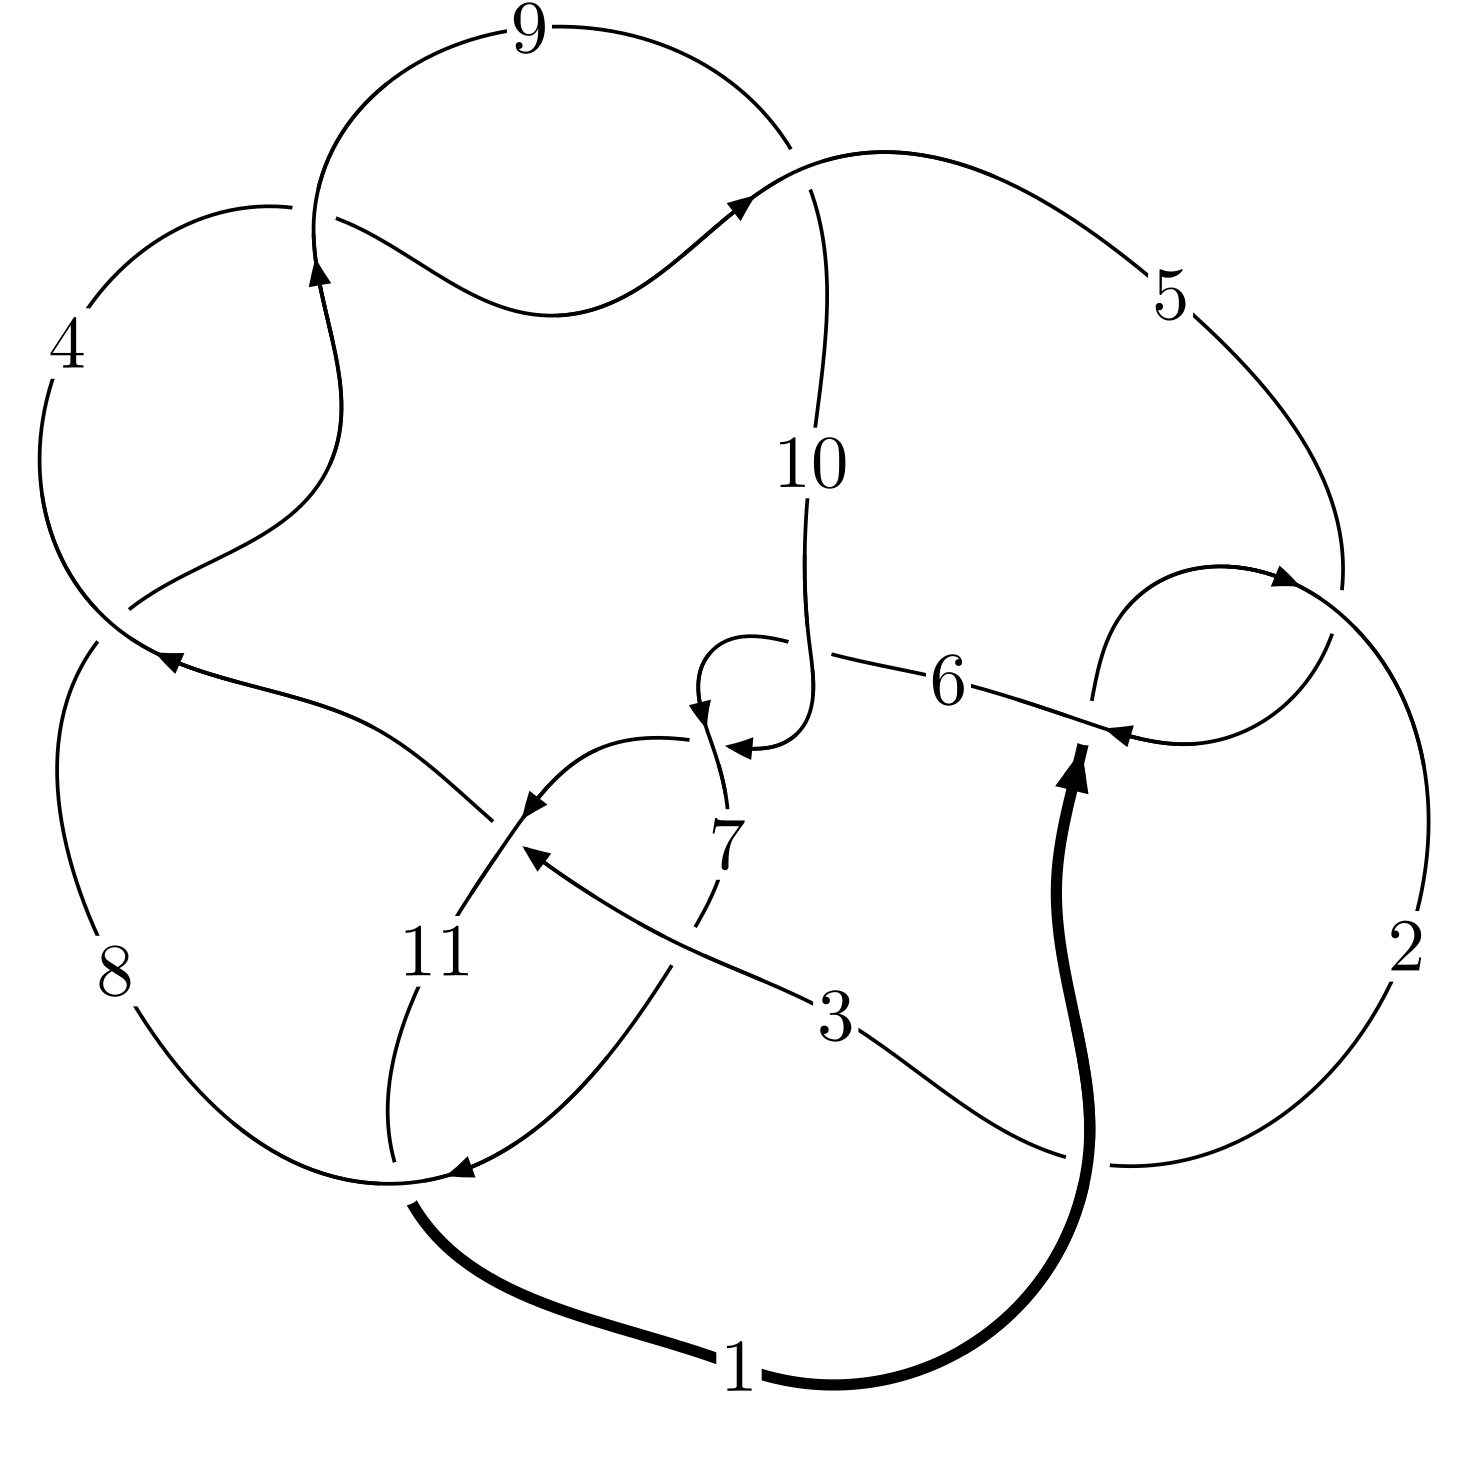
\includegraphics[width=112pt]{../../../GIT/diagram.site/Diagrams/png/362_11a_113.png}\\
\ \ \ A knot diagram\footnotemark}&
\allowdisplaybreaks
\textbf{Linearized knot diagam} \\
\cline{2-2}
 &
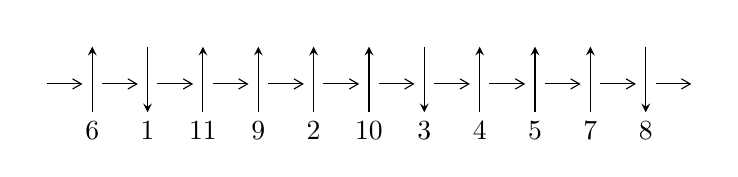
\begin{tikzpicture}[x=20pt, y=17pt]
	% nodes
	\node (C0) at (0, 0) {};
	\node (C1) at (1, 0) {};
	\node (C1U) at (1, +1) {};
	\node (C1D) at (1, -1) {6};

	\node (C2) at (2, 0) {};
	\node (C2U) at (2, +1) {};
	\node (C2D) at (2, -1) {1};

	\node (C3) at (3, 0) {};
	\node (C3U) at (3, +1) {};
	\node (C3D) at (3, -1) {11};

	\node (C4) at (4, 0) {};
	\node (C4U) at (4, +1) {};
	\node (C4D) at (4, -1) {9};

	\node (C5) at (5, 0) {};
	\node (C5U) at (5, +1) {};
	\node (C5D) at (5, -1) {2};

	\node (C6) at (6, 0) {};
	\node (C6U) at (6, +1) {};
	\node (C6D) at (6, -1) {10};

	\node (C7) at (7, 0) {};
	\node (C7U) at (7, +1) {};
	\node (C7D) at (7, -1) {3};

	\node (C8) at (8, 0) {};
	\node (C8U) at (8, +1) {};
	\node (C8D) at (8, -1) {4};

	\node (C9) at (9, 0) {};
	\node (C9U) at (9, +1) {};
	\node (C9D) at (9, -1) {5};

	\node (C10) at (10, 0) {};
	\node (C10U) at (10, +1) {};
	\node (C10D) at (10, -1) {7};

	\node (C11) at (11, 0) {};
	\node (C11U) at (11, +1) {};
	\node (C11D) at (11, -1) {8};
	\node (C12) at (12, 0) {};

	% arrows
	\draw[->,>={angle 60}]
	(C0) edge (C1) (C1) edge (C2) (C2) edge (C3) (C3) edge (C4) (C4) edge (C5) (C5) edge (C6) (C6) edge (C7) (C7) edge (C8) (C8) edge (C9) (C9) edge (C10) (C10) edge (C11) (C11) edge (C12) ;	\draw[->,>=stealth]
	(C1D) edge (C1U) (C2U) edge (C2D) (C3D) edge (C3U) (C4D) edge (C4U) (C5D) edge (C5U) (C6D) edge (C6U) (C7U) edge (C7D) (C8D) edge (C8U) (C9D) edge (C9U) (C10D) edge (C10U) (C11U) edge (C11D) ;
	\end{tikzpicture} \\
\hhline{~~} \\& 
\textbf{Solving Sequence} \\ \cline{2-2} 
 &
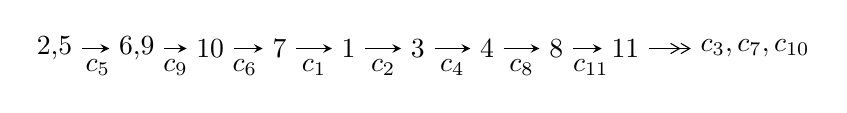
\begin{tikzpicture}[x=25pt, y=7pt]
	% node
	\node (A0) at (-1/8, 0) {2,5};
	\node (A1) at (17/16, 0) {6,9};
	\node (A2) at (17/8, 0) {10};
	\node (A3) at (25/8, 0) {7};
	\node (A4) at (33/8, 0) {1};
	\node (A5) at (41/8, 0) {3};
	\node (A6) at (49/8, 0) {4};
	\node (A7) at (57/8, 0) {8};
	\node (A8) at (65/8, 0) {11};
	\node (C1) at (1/2, -1) {$c_{5}$};
	\node (C2) at (13/8, -1) {$c_{9}$};
	\node (C3) at (21/8, -1) {$c_{6}$};
	\node (C4) at (29/8, -1) {$c_{1}$};
	\node (C5) at (37/8, -1) {$c_{2}$};
	\node (C6) at (45/8, -1) {$c_{4}$};
	\node (C7) at (53/8, -1) {$c_{8}$};
	\node (C8) at (61/8, -1) {$c_{11}$};
	\node (A9) at (10, 0) {$c_{3},c_{7},c_{10}$};

	% edge
	\draw[->,>=stealth]	
	(A0) edge (A1) (A1) edge (A2) (A2) edge (A3) (A3) edge (A4) (A4) edge (A5) (A5) edge (A6) (A6) edge (A7) (A7) edge (A8) ;
	\draw[->>,>={angle 60}]	
	(A8) edge (A9);
\end{tikzpicture} \\ 

\end{tabular} \\

\footnotetext{
The image of knot diagram is generated by the software ``\textbf{Draw programme}" developed by Andrew Bartholomew(\url{http://www.layer8.co.uk/maths/draw/index.htm\#Running-draw}), where we modified some parts for our purpose(\url{https://github.com/CATsTAILs/LinksPainter}).
}\phantom \\ \newline 
\centering \textbf{Ideals for irreducible components\footnotemark of $X_{\text{par}}$} 
 
\begin{align*}
I^u_{1}&=\langle 
5.34839\times10^{80} u^{67}+3.68124\times10^{80} u^{66}+\cdots+1.27153\times10^{82} b-1.90765\times10^{82},\\
\phantom{I^u_{1}}&\phantom{= \langle  }6.93735\times10^{81} u^{67}-9.19994\times10^{80} u^{66}+\cdots+1.27153\times10^{82} a-4.71008\times10^{82},\;u^{68}+12 u^{66}+\cdots+14 u+1\rangle \\
I^u_{2}&=\langle 
u^{12}+3 u^{10}+7 u^8+9 u^6+u^5+8 u^4+2 u^3+4 u^2+b+u+2,\\
\phantom{I^u_{2}}&\phantom{= \langle  }u^{13}+3 u^{12}+6 u^{11}+10 u^{10}+14 u^9+20 u^8+22 u^7+25 u^6+23 u^5+22 u^4+17 u^3+11 u^2+a+4 u+3,\\
\phantom{I^u_{2}}&\phantom{= \langle  }u^{14}+u^{13}+4 u^{12}+3 u^{11}+9 u^{10}+6 u^9+13 u^8+8 u^7+13 u^6+8 u^5+9 u^4+4 u^3+4 u^2+u+1\rangle \\
\\
\end{align*}
\raggedright * 2 irreducible components of $\dim_{\mathbb{C}}=0$, with total 82 representations.\\
\footnotetext{All coefficients of polynomials are rational numbers. But the coefficients are sometimes approximated in decimal forms when there is not enough margin.}
\newpage
\renewcommand{\arraystretch}{1}
\centering \section*{I. $I^u_{1}= \langle 5.35\times10^{80} u^{67}+3.68\times10^{80} u^{66}+\cdots+1.27\times10^{82} b-1.91\times10^{82},\;6.94\times10^{81} u^{67}-9.20\times10^{80} u^{66}+\cdots+1.27\times10^{82} a-4.71\times10^{82},\;u^{68}+12 u^{66}+\cdots+14 u+1 \rangle$}
\flushleft \textbf{(i) Arc colorings}\\
\begin{tabular}{m{7pt} m{180pt} m{7pt} m{180pt} }
\flushright $a_{2}=$&$\begin{pmatrix}0\\u\end{pmatrix}$ \\
\flushright $a_{5}=$&$\begin{pmatrix}1\\0\end{pmatrix}$ \\
\flushright $a_{6}=$&$\begin{pmatrix}1\\- u^2\end{pmatrix}$ \\
\flushright $a_{9}=$&$\begin{pmatrix}-0.545593 u^{67}+0.0723536 u^{66}+\cdots-2.02184 u+3.70427\\-0.0420628 u^{67}-0.0289514 u^{66}+\cdots-1.69314 u+1.50029\end{pmatrix}$ \\
\flushright $a_{10}=$&$\begin{pmatrix}-0.587656 u^{67}+0.0434022 u^{66}+\cdots-3.71498 u+5.20456\\-0.0420628 u^{67}-0.0289514 u^{66}+\cdots-1.69314 u+1.50029\end{pmatrix}$ \\
\flushright $a_{7}=$&$\begin{pmatrix}-0.355881 u^{67}+0.380128 u^{66}+\cdots+8.26080 u-6.73774\\-0.194171 u^{67}+0.115092 u^{66}+\cdots-1.69115 u-2.69071\end{pmatrix}$ \\
\flushright $a_{1}=$&$\begin{pmatrix}- u\\u^3+u\end{pmatrix}$ \\
\flushright $a_{3}=$&$\begin{pmatrix}- u^3\\u^5+u^3+u\end{pmatrix}$ \\
\flushright $a_{4}=$&$\begin{pmatrix}-0.444897 u^{67}-0.0337046 u^{66}+\cdots-7.30208 u+6.51254\\0.126760 u^{67}-0.101224 u^{66}+\cdots-0.515987 u+2.55578\end{pmatrix}$ \\
\flushright $a_{8}=$&$\begin{pmatrix}-0.322518 u^{67}+0.382112 u^{66}+\cdots+7.92528 u-6.76024\\-0.224672 u^{67}+0.0956000 u^{66}+\cdots-5.25233 u-2.97848\end{pmatrix}$ \\
\flushright $a_{11}=$&$\begin{pmatrix}-1.65034 u^{67}+0.264278 u^{66}+\cdots-36.4509 u-9.08954\\-0.600905 u^{67}+0.0210170 u^{66}+\cdots-17.9861 u-3.94419\end{pmatrix}$\\ \flushright $a_{11}=$&$\begin{pmatrix}-1.65034 u^{67}+0.264278 u^{66}+\cdots-36.4509 u-9.08954\\-0.600905 u^{67}+0.0210170 u^{66}+\cdots-17.9861 u-3.94419\end{pmatrix}$\\&\end{tabular}
\flushleft \textbf{(ii) Obstruction class $= -1$}\\~\\
\flushleft \textbf{(iii) Cusp Shapes $= -1.99975 u^{67}+0.337333 u^{66}+\cdots-36.0266 u-0.689887$}\\~\\
\newpage\renewcommand{\arraystretch}{1}
\flushleft \textbf{(iv) u-Polynomials at the component}\newline \\
\begin{tabular}{m{50pt}|m{274pt}}
Crossings & \hspace{64pt}u-Polynomials at each crossing \\
\hline $$\begin{aligned}c_{1},c_{5}\end{aligned}$$&$\begin{aligned}
&u^{68}+12 u^{66}+\cdots-14 u+1
\end{aligned}$\\
\hline $$\begin{aligned}c_{2}\end{aligned}$$&$\begin{aligned}
&u^{68}+24 u^{67}+\cdots-66 u+1
\end{aligned}$\\
\hline $$\begin{aligned}c_{3}\end{aligned}$$&$\begin{aligned}
&u^{68}+5 u^{67}+\cdots+1376 u+161
\end{aligned}$\\
\hline $$\begin{aligned}c_{4},c_{8},c_{9}\end{aligned}$$&$\begin{aligned}
&u^{68}+u^{67}+\cdots-13 u-19
\end{aligned}$\\
\hline $$\begin{aligned}c_{6},c_{10}\end{aligned}$$&$\begin{aligned}
&u^{68}+u^{67}+\cdots+99 u-13
\end{aligned}$\\
\hline $$\begin{aligned}c_{7}\end{aligned}$$&$\begin{aligned}
&u^{68}- u^{67}+\cdots-83 u-123
\end{aligned}$\\
\hline $$\begin{aligned}c_{11}\end{aligned}$$&$\begin{aligned}
&u^{68}+5 u^{67}+\cdots-131 u-179
\end{aligned}$\\
\hline
\end{tabular}\\~\\
\newpage\renewcommand{\arraystretch}{1}
\flushleft \textbf{(v) Riley Polynomials at the component}\newline \\
\begin{tabular}{m{50pt}|m{274pt}}
Crossings & \hspace{64pt}Riley Polynomials at each crossing \\
\hline $$\begin{aligned}c_{1},c_{5}\end{aligned}$$&$\begin{aligned}
&y^{68}+24 y^{67}+\cdots-66 y+1
\end{aligned}$\\
\hline $$\begin{aligned}c_{2}\end{aligned}$$&$\begin{aligned}
&y^{68}+48 y^{67}+\cdots-11082 y+1
\end{aligned}$\\
\hline $$\begin{aligned}c_{3}\end{aligned}$$&$\begin{aligned}
&y^{68}-23 y^{67}+\cdots-1710480 y+25921
\end{aligned}$\\
\hline $$\begin{aligned}c_{4},c_{8},c_{9}\end{aligned}$$&$\begin{aligned}
&y^{68}-75 y^{67}+\cdots-1537 y+361
\end{aligned}$\\
\hline $$\begin{aligned}c_{6},c_{10}\end{aligned}$$&$\begin{aligned}
&y^{68}-61 y^{67}+\cdots+17369 y+169
\end{aligned}$\\
\hline $$\begin{aligned}c_{7}\end{aligned}$$&$\begin{aligned}
&y^{68}+17 y^{67}+\cdots+422135 y+15129
\end{aligned}$\\
\hline $$\begin{aligned}c_{11}\end{aligned}$$&$\begin{aligned}
&y^{68}+21 y^{67}+\cdots+1105527 y+32041
\end{aligned}$\\
\hline
\end{tabular}\\~\\
\newpage\flushleft \textbf{(vi) Complex Volumes and Cusp Shapes}
$$\begin{array}{c|c|c}  
\text{Solutions to }I^u_{1}& \I (\text{vol} + \sqrt{-1}CS) & \text{Cusp shape}\\
 \hline 
\begin{aligned}
u &= \phantom{-}0.056691 + 0.998319 I \\
a &= \phantom{-}0.429493 - 0.794328 I \\
b &= -1.354540 - 0.227994 I\end{aligned}
 & \phantom{-}1.84313 + 3.63375 I & \phantom{-}5.00000 + 0. I\phantom{ +0.000000I} \\ \hline\begin{aligned}
u &= \phantom{-}0.056691 - 0.998319 I \\
a &= \phantom{-}0.429493 + 0.794328 I \\
b &= -1.354540 + 0.227994 I\end{aligned}
 & \phantom{-}1.84313 - 3.63375 I & \phantom{-}5.00000 + 0. I\phantom{ +0.000000I} \\ \hline\begin{aligned}
u &= -0.737376 + 0.671219 I \\
a &= -2.08721 + 0.27350 I \\
b &= \phantom{-}1.58093 + 0.06731 I\end{aligned}
 & \phantom{-}11.54460 + 0.21877 I & \phantom{-}17.6771 + 0. I\phantom{ +0.000000I} \\ \hline\begin{aligned}
u &= -0.737376 - 0.671219 I \\
a &= -2.08721 - 0.27350 I \\
b &= \phantom{-}1.58093 - 0.06731 I\end{aligned}
 & \phantom{-}11.54460 - 0.21877 I & \phantom{-}17.6771 + 0. I\phantom{ +0.000000I} \\ \hline\begin{aligned}
u &= \phantom{-}0.124547 + 0.983422 I \\
a &= \phantom{-}0.010360 - 0.721178 I \\
b &= \phantom{-}0.219106 - 0.623961 I\end{aligned}
 & -3.12233 - 0.57125 I & \phantom{-0.000000 } 0 \\ \hline\begin{aligned}
u &= \phantom{-}0.124547 - 0.983422 I \\
a &= \phantom{-}0.010360 + 0.721178 I \\
b &= \phantom{-}0.219106 + 0.623961 I\end{aligned}
 & -3.12233 + 0.57125 I & \phantom{-0.000000 } 0 \\ \hline\begin{aligned}
u &= -0.350162 + 0.974636 I \\
a &= -0.417402 - 1.047070 I \\
b &= \phantom{-}0.832916 - 0.285678 I\end{aligned}
 & -1.26804 - 2.79796 I & \phantom{-0.000000 } 0 \\ \hline\begin{aligned}
u &= -0.350162 - 0.974636 I \\
a &= -0.417402 + 1.047070 I \\
b &= \phantom{-}0.832916 + 0.285678 I\end{aligned}
 & -1.26804 + 2.79796 I & \phantom{-0.000000 } 0 \\ \hline\begin{aligned}
u &= \phantom{-}0.786533 + 0.684928 I \\
a &= -1.66355 + 0.54319 I \\
b &= \phantom{-}1.72387 - 0.29020 I\end{aligned}
 & \phantom{-}12.09960 - 0.83840 I & \phantom{-0.000000 } 0 \\ \hline\begin{aligned}
u &= \phantom{-}0.786533 - 0.684928 I \\
a &= -1.66355 - 0.54319 I \\
b &= \phantom{-}1.72387 + 0.29020 I\end{aligned}
 & \phantom{-}12.09960 + 0.83840 I & \phantom{-0.000000 } 0\\
 \hline 
 \end{array}$$\newpage$$\begin{array}{c|c|c}  
\text{Solutions to }I^u_{1}& \I (\text{vol} + \sqrt{-1}CS) & \text{Cusp shape}\\
 \hline 
\begin{aligned}
u &= \phantom{-}0.830250 + 0.658865 I \\
a &= -0.250221 + 0.410875 I \\
b &= \phantom{-}0.798752 - 0.772203 I\end{aligned}
 & \phantom{-}5.67993 - 5.34809 I & \phantom{-0.000000 } 0 \\ \hline\begin{aligned}
u &= \phantom{-}0.830250 - 0.658865 I \\
a &= -0.250221 - 0.410875 I \\
b &= \phantom{-}0.798752 + 0.772203 I\end{aligned}
 & \phantom{-}5.67993 + 5.34809 I & \phantom{-0.000000 } 0 \\ \hline\begin{aligned}
u &= -0.749134 + 0.751065 I \\
a &= -2.64257 - 0.98796 I \\
b &= \phantom{-}1.50979 + 0.07061 I\end{aligned}
 & \phantom{-}7.17486 + 3.06656 I & \phantom{-0.000000 } 0 \\ \hline\begin{aligned}
u &= -0.749134 - 0.751065 I \\
a &= -2.64257 + 0.98796 I \\
b &= \phantom{-}1.50979 - 0.07061 I\end{aligned}
 & \phantom{-}7.17486 - 3.06656 I & \phantom{-0.000000 } 0 \\ \hline\begin{aligned}
u &= -0.906668 + 0.562915 I \\
a &= -0.063631 + 0.203600 I \\
b &= \phantom{-}0.565448 + 0.170026 I\end{aligned}
 & \phantom{-}4.68598 - 2.04595 I & \phantom{-0.000000 } 0 \\ \hline\begin{aligned}
u &= -0.906668 - 0.562915 I \\
a &= -0.063631 - 0.203600 I \\
b &= \phantom{-}0.565448 - 0.170026 I\end{aligned}
 & \phantom{-}4.68598 + 2.04595 I & \phantom{-0.000000 } 0 \\ \hline\begin{aligned}
u &= \phantom{-}0.789964 + 0.729685 I \\
a &= -2.20736 + 1.00128 I \\
b &= \phantom{-}1.50674 + 0.17499 I\end{aligned}
 & \phantom{-}7.19896 + 3.40495 I & \phantom{-0.000000 } 0 \\ \hline\begin{aligned}
u &= \phantom{-}0.789964 - 0.729685 I \\
a &= -2.20736 - 1.00128 I \\
b &= \phantom{-}1.50674 - 0.17499 I\end{aligned}
 & \phantom{-}7.19896 - 3.40495 I & \phantom{-0.000000 } 0 \\ \hline\begin{aligned}
u &= -0.024461 + 1.086200 I \\
a &= -0.840798 - 0.156923 I \\
b &= -1.47061 + 0.12446 I\end{aligned}
 & \phantom{-}6.24502 - 0.43169 I & \phantom{-0.000000 } 0 \\ \hline\begin{aligned}
u &= -0.024461 - 1.086200 I \\
a &= -0.840798 + 0.156923 I \\
b &= -1.47061 - 0.12446 I\end{aligned}
 & \phantom{-}6.24502 + 0.43169 I & \phantom{-0.000000 } 0\\
 \hline 
 \end{array}$$\newpage$$\begin{array}{c|c|c}  
\text{Solutions to }I^u_{1}& \I (\text{vol} + \sqrt{-1}CS) & \text{Cusp shape}\\
 \hline 
\begin{aligned}
u &= \phantom{-}0.668707 + 0.865207 I \\
a &= \phantom{-}0.704861 + 0.333087 I \\
b &= -0.616750 + 0.357372 I\end{aligned}
 & \phantom{-}4.01661 + 1.17981 I & \phantom{-0.000000 } 0 \\ \hline\begin{aligned}
u &= \phantom{-}0.668707 - 0.865207 I \\
a &= \phantom{-}0.704861 - 0.333087 I \\
b &= -0.616750 - 0.357372 I\end{aligned}
 & \phantom{-}4.01661 - 1.17981 I & \phantom{-0.000000 } 0 \\ \hline\begin{aligned}
u &= \phantom{-}0.679050 + 0.858235 I \\
a &= -0.77402 + 1.29486 I \\
b &= \phantom{-}0.400623 + 0.354831 I\end{aligned}
 & \phantom{-}4.03879 + 4.03484 I & \phantom{-0.000000 } 0 \\ \hline\begin{aligned}
u &= \phantom{-}0.679050 - 0.858235 I \\
a &= -0.77402 - 1.29486 I \\
b &= \phantom{-}0.400623 - 0.354831 I\end{aligned}
 & \phantom{-}4.03879 - 4.03484 I & \phantom{-0.000000 } 0 \\ \hline\begin{aligned}
u &= -0.710320 + 0.840348 I \\
a &= -1.094730 - 0.412872 I \\
b &= \phantom{-}0.418566 - 1.103500 I\end{aligned}
 & \phantom{-}4.26526 - 0.78149 I & \phantom{-0.000000 } 0 \\ \hline\begin{aligned}
u &= -0.710320 - 0.840348 I \\
a &= -1.094730 + 0.412872 I \\
b &= \phantom{-}0.418566 + 1.103500 I\end{aligned}
 & \phantom{-}4.26526 + 0.78149 I & \phantom{-0.000000 } 0 \\ \hline\begin{aligned}
u &= -0.703267 + 0.893390 I \\
a &= -0.176298 + 0.303056 I \\
b &= -0.611742 - 1.091160 I\end{aligned}
 & \phantom{-}4.10083 - 4.63563 I & \phantom{-0.000000 } 0 \\ \hline\begin{aligned}
u &= -0.703267 - 0.893390 I \\
a &= -0.176298 - 0.303056 I \\
b &= -0.611742 + 1.091160 I\end{aligned}
 & \phantom{-}4.10083 + 4.63563 I & \phantom{-0.000000 } 0 \\ \hline\begin{aligned}
u &= \phantom{-}0.564977 + 0.999135 I \\
a &= -1.220080 + 0.538963 I \\
b &= \phantom{-}0.536796 + 0.482587 I\end{aligned}
 & -0.51569 + 6.32863 I & \phantom{-0.000000 } 0 \\ \hline\begin{aligned}
u &= \phantom{-}0.564977 - 0.999135 I \\
a &= -1.220080 - 0.538963 I \\
b &= \phantom{-}0.536796 - 0.482587 I\end{aligned}
 & -0.51569 - 6.32863 I & \phantom{-0.000000 } 0\\
 \hline 
 \end{array}$$\newpage$$\begin{array}{c|c|c}  
\text{Solutions to }I^u_{1}& \I (\text{vol} + \sqrt{-1}CS) & \text{Cusp shape}\\
 \hline 
\begin{aligned}
u &= -0.493291 + 1.042080 I \\
a &= -0.032396 - 0.417531 I \\
b &= \phantom{-}0.538420 + 0.338146 I\end{aligned}
 & -0.59382 - 3.25955 I & \phantom{-0.000000 } 0 \\ \hline\begin{aligned}
u &= -0.493291 - 1.042080 I \\
a &= -0.032396 + 0.417531 I \\
b &= \phantom{-}0.538420 - 0.338146 I\end{aligned}
 & -0.59382 + 3.25955 I & \phantom{-0.000000 } 0 \\ \hline\begin{aligned}
u &= -0.152408 + 1.170190 I \\
a &= -0.442695 + 0.367195 I \\
b &= -0.308154 + 0.476045 I\end{aligned}
 & -1.12613 - 4.69478 I & \phantom{-0.000000 } 0 \\ \hline\begin{aligned}
u &= -0.152408 - 1.170190 I \\
a &= -0.442695 - 0.367195 I \\
b &= -0.308154 - 0.476045 I\end{aligned}
 & -1.12613 + 4.69478 I & \phantom{-0.000000 } 0 \\ \hline\begin{aligned}
u &= -0.709893 + 0.967350 I \\
a &= \phantom{-}2.26969 + 1.36925 I \\
b &= -1.55119 + 0.14708 I\end{aligned}
 & \phantom{-}6.51252 - 8.62631 I & \phantom{-0.000000 } 0 \\ \hline\begin{aligned}
u &= -0.709893 - 0.967350 I \\
a &= \phantom{-}2.26969 - 1.36925 I \\
b &= -1.55119 - 0.14708 I\end{aligned}
 & \phantom{-}6.51252 + 8.62631 I & \phantom{-0.000000 } 0 \\ \hline\begin{aligned}
u &= -0.072290 + 0.784893 I \\
a &= \phantom{-}1.44712 + 1.00338 I \\
b &= -0.867537 + 0.492868 I\end{aligned}
 & \phantom{-}0.479696 + 1.218850 I & \phantom{-}3.82242 - 2.62908 I \\ \hline\begin{aligned}
u &= -0.072290 - 0.784893 I \\
a &= \phantom{-}1.44712 - 1.00338 I \\
b &= -0.867537 - 0.492868 I\end{aligned}
 & \phantom{-}0.479696 - 1.218850 I & \phantom{-}3.82242 + 2.62908 I \\ \hline\begin{aligned}
u &= -1.036660 + 0.628687 I \\
a &= \phantom{-}1.76825 + 0.21237 I \\
b &= -1.62760 - 0.23134 I\end{aligned}
 & \phantom{-}13.7366 + 9.0871 I & \phantom{-0.000000 } 0 \\ \hline\begin{aligned}
u &= -1.036660 - 0.628687 I \\
a &= \phantom{-}1.76825 - 0.21237 I \\
b &= -1.62760 + 0.23134 I\end{aligned}
 & \phantom{-}13.7366 - 9.0871 I & \phantom{-0.000000 } 0\\
 \hline 
 \end{array}$$\newpage$$\begin{array}{c|c|c}  
\text{Solutions to }I^u_{1}& \I (\text{vol} + \sqrt{-1}CS) & \text{Cusp shape}\\
 \hline 
\begin{aligned}
u &= -0.687079 + 1.010450 I \\
a &= \phantom{-}1.32026 + 2.12559 I \\
b &= -1.51603 + 0.10725 I\end{aligned}
 & \phantom{-}10.52170 - 5.68294 I & \phantom{-0.000000 } 0 \\ \hline\begin{aligned}
u &= -0.687079 - 1.010450 I \\
a &= \phantom{-}1.32026 - 2.12559 I \\
b &= -1.51603 - 0.10725 I\end{aligned}
 & \phantom{-}10.52170 + 5.68294 I & \phantom{-0.000000 } 0 \\ \hline\begin{aligned}
u &= \phantom{-}0.742606 + 0.989112 I \\
a &= \phantom{-}1.71217 - 0.97802 I \\
b &= -1.52663 + 0.03900 I\end{aligned}
 & \phantom{-}6.41405 + 2.38016 I & \phantom{-0.000000 } 0 \\ \hline\begin{aligned}
u &= \phantom{-}0.742606 - 0.989112 I \\
a &= \phantom{-}1.71217 + 0.97802 I \\
b &= -1.52663 - 0.03900 I\end{aligned}
 & \phantom{-}6.41405 - 2.38016 I & \phantom{-0.000000 } 0 \\ \hline\begin{aligned}
u &= \phantom{-}0.560580 + 0.511556 I \\
a &= \phantom{-}1.077470 - 0.460333 I \\
b &= -0.359314 + 0.358132 I\end{aligned}
 & \phantom{-}0.85594 - 1.76487 I & \phantom{-}7.42480 + 4.84873 I \\ \hline\begin{aligned}
u &= \phantom{-}0.560580 - 0.511556 I \\
a &= \phantom{-}1.077470 + 0.460333 I \\
b &= -0.359314 - 0.358132 I\end{aligned}
 & \phantom{-}0.85594 + 1.76487 I & \phantom{-}7.42480 - 4.84873 I \\ \hline\begin{aligned}
u &= \phantom{-}0.713931 + 1.015970 I \\
a &= \phantom{-}1.41258 - 1.55830 I \\
b &= -1.65304 - 0.39573 I\end{aligned}
 & \phantom{-}11.09840 + 6.52113 I & \phantom{-0.000000 } 0 \\ \hline\begin{aligned}
u &= \phantom{-}0.713931 - 1.015970 I \\
a &= \phantom{-}1.41258 + 1.55830 I \\
b &= -1.65304 + 0.39573 I\end{aligned}
 & \phantom{-}11.09840 - 6.52113 I & \phantom{-0.000000 } 0 \\ \hline\begin{aligned}
u &= \phantom{-}0.725112 + 1.032960 I \\
a &= \phantom{-}1.016130 - 0.612765 I \\
b &= -0.696435 - 0.914112 I\end{aligned}
 & \phantom{-}4.55307 + 11.17470 I & \phantom{-0.000000 } 0 \\ \hline\begin{aligned}
u &= \phantom{-}0.725112 - 1.032960 I \\
a &= \phantom{-}1.016130 + 0.612765 I \\
b &= -0.696435 + 0.914112 I\end{aligned}
 & \phantom{-}4.55307 - 11.17470 I & \phantom{-0.000000 } 0\\
 \hline 
 \end{array}$$\newpage$$\begin{array}{c|c|c}  
\text{Solutions to }I^u_{1}& \I (\text{vol} + \sqrt{-1}CS) & \text{Cusp shape}\\
 \hline 
\begin{aligned}
u &= -0.506212 + 0.514162 I \\
a &= \phantom{-}1.000830 - 0.052860 I \\
b &= -0.358987 + 0.452126 I\end{aligned}
 & \phantom{-}1.004420 - 0.901476 I & \phantom{-}8.36804 + 5.20975 I \\ \hline\begin{aligned}
u &= -0.506212 - 0.514162 I \\
a &= \phantom{-}1.000830 + 0.052860 I \\
b &= -0.358987 - 0.452126 I\end{aligned}
 & \phantom{-}1.004420 + 0.901476 I & \phantom{-}8.36804 - 5.20975 I \\ \hline\begin{aligned}
u &= -0.772141 + 1.064070 I \\
a &= \phantom{-}0.404218 + 0.523737 I \\
b &= -0.378482 + 0.463468 I\end{aligned}
 & \phantom{-}3.24077 - 4.14481 I & \phantom{-0.000000 } 0 \\ \hline\begin{aligned}
u &= -0.772141 - 1.064070 I \\
a &= \phantom{-}0.404218 - 0.523737 I \\
b &= -0.378482 - 0.463468 I\end{aligned}
 & \phantom{-}3.24077 + 4.14481 I & \phantom{-0.000000 } 0 \\ \hline\begin{aligned}
u &= \phantom{-}1.281700 + 0.464275 I \\
a &= \phantom{-}1.66046 - 0.06858 I \\
b &= -1.54861 + 0.02461 I\end{aligned}
 & \phantom{-}11.85000 + 1.49284 I & \phantom{-0.000000 } 0 \\ \hline\begin{aligned}
u &= \phantom{-}1.281700 - 0.464275 I \\
a &= \phantom{-}1.66046 + 0.06858 I \\
b &= -1.54861 - 0.02461 I\end{aligned}
 & \phantom{-}11.85000 - 1.49284 I & \phantom{-0.000000 } 0 \\ \hline\begin{aligned}
u &= -0.784798 + 1.129230 I \\
a &= -1.46411 - 1.43292 I \\
b &= \phantom{-}1.61931 - 0.29900 I\end{aligned}
 & \phantom{-}12.1505 - 15.6778 I & \phantom{-0.000000 } 0 \\ \hline\begin{aligned}
u &= -0.784798 - 1.129230 I \\
a &= -1.46411 + 1.43292 I \\
b &= \phantom{-}1.61931 + 0.29900 I\end{aligned}
 & \phantom{-}12.1505 + 15.6778 I & \phantom{-0.000000 } 0 \\ \hline\begin{aligned}
u &= \phantom{-}0.035097 + 0.578937 I \\
a &= \phantom{-}2.16601 - 0.21856 I \\
b &= \phantom{-}0.030110 + 0.376253 I\end{aligned}
 & \phantom{-}0.96062 - 1.38974 I & \phantom{-}4.85505 + 5.15507 I \\ \hline\begin{aligned}
u &= \phantom{-}0.035097 - 0.578937 I \\
a &= \phantom{-}2.16601 + 0.21856 I \\
b &= \phantom{-}0.030110 - 0.376253 I\end{aligned}
 & \phantom{-}0.96062 + 1.38974 I & \phantom{-}4.85505 - 5.15507 I\\
 \hline 
 \end{array}$$\newpage$$\begin{array}{c|c|c}  
\text{Solutions to }I^u_{1}& \I (\text{vol} + \sqrt{-1}CS) & \text{Cusp shape}\\
 \hline 
\begin{aligned}
u &= \phantom{-}0.22199 + 1.44135 I \\
a &= -0.308371 + 0.423417 I \\
b &= \phantom{-}1.49524 + 0.11629 I\end{aligned}
 & \phantom{-}4.95386 + 6.63333 I & \phantom{-0.000000 } 0 \\ \hline\begin{aligned}
u &= \phantom{-}0.22199 - 1.44135 I \\
a &= -0.308371 - 0.423417 I \\
b &= \phantom{-}1.49524 - 0.11629 I\end{aligned}
 & \phantom{-}4.95386 - 6.63333 I & \phantom{-0.000000 } 0 \\ \hline\begin{aligned}
u &= \phantom{-}0.91649 + 1.24644 I \\
a &= -1.34038 + 1.01266 I \\
b &= \phantom{-}1.49909 + 0.12802 I\end{aligned}
 & \phantom{-}9.50152 + 6.18867 I & \phantom{-0.000000 } 0 \\ \hline\begin{aligned}
u &= \phantom{-}0.91649 - 1.24644 I \\
a &= -1.34038 - 1.01266 I \\
b &= \phantom{-}1.49909 - 0.12802 I\end{aligned}
 & \phantom{-}9.50152 - 6.18867 I & \phantom{-0.000000 } 0 \\ \hline\begin{aligned}
u &= -0.422490\phantom{ +0.000000I} \\
a &= \phantom{-}1.36125\phantom{ +0.000000I} \\
b &= -0.753301\phantom{ +0.000000I}\end{aligned}
 & \phantom{-}1.14898\phantom{ +0.000000I} & \phantom{-}8.76770\phantom{ +0.000000I} \\ \hline\begin{aligned}
u &= -0.041792 + 0.289775 I \\
a &= \phantom{-}4.68550 + 1.04734 I \\
b &= \phantom{-}1.215190 - 0.166969 I\end{aligned}
 & \phantom{-}4.61196 - 3.48976 I & \phantom{-}13.3589 + 6.7779 I \\ \hline\begin{aligned}
u &= -0.041792 - 0.289775 I \\
a &= \phantom{-}4.68550 - 1.04734 I \\
b &= \phantom{-}1.215190 + 0.166969 I\end{aligned}
 & \phantom{-}4.61196 + 3.48976 I & \phantom{-}13.3589 - 6.7779 I \\ \hline\begin{aligned}
u &= -0.0980352\phantom{ +0.000000I} \\
a &= \phantom{-}3.51954\phantom{ +0.000000I} \\
b &= \phantom{-}1.66282\phantom{ +0.000000I}\end{aligned}
 & \phantom{-}10.1505\phantom{ +0.000000I} & -0.505670\phantom{ +0.000000I}\\
 \hline 
 \end{array}$$\newpage\newpage\renewcommand{\arraystretch}{1}
\centering \section*{II. $I^u_{2}= \langle u^{12}+3 u^{10}+\cdots+b+2,\;u^{13}+3 u^{12}+\cdots+a+3,\;u^{14}+u^{13}+\cdots+u+1 \rangle$}
\flushleft \textbf{(i) Arc colorings}\\
\begin{tabular}{m{7pt} m{180pt} m{7pt} m{180pt} }
\flushright $a_{2}=$&$\begin{pmatrix}0\\u\end{pmatrix}$ \\
\flushright $a_{5}=$&$\begin{pmatrix}1\\0\end{pmatrix}$ \\
\flushright $a_{6}=$&$\begin{pmatrix}1\\- u^2\end{pmatrix}$ \\
\flushright $a_{9}=$&$\begin{pmatrix}- u^{13}-3 u^{12}+\cdots-4 u-3\\- u^{12}-3 u^{10}-7 u^8-9 u^6- u^5-8 u^4-2 u^3-4 u^2- u-2\end{pmatrix}$ \\
\flushright $a_{10}=$&$\begin{pmatrix}- u^{13}-4 u^{12}+\cdots-5 u-5\\- u^{12}-3 u^{10}-7 u^8-9 u^6- u^5-8 u^4-2 u^3-4 u^2- u-2\end{pmatrix}$ \\
\flushright $a_{7}=$&$\begin{pmatrix}2 u^{13}+2 u^{12}+\cdots+u+2\\u^{13}+2 u^{12}+\cdots+2 u+1\end{pmatrix}$ \\
\flushright $a_{1}=$&$\begin{pmatrix}- u\\u^3+u\end{pmatrix}$ \\
\flushright $a_{3}=$&$\begin{pmatrix}- u^3\\u^5+u^3+u\end{pmatrix}$ \\
\flushright $a_{4}=$&$\begin{pmatrix}u^{13}+4 u^{12}+\cdots+2 u+4\\u^{13}+u^{12}+\cdots+3 u+2\end{pmatrix}$ \\
\flushright $a_{8}=$&$\begin{pmatrix}u^{13}+u^{12}+2 u^{11}+u^{10}+3 u^9+2 u^8+2 u^7+u^6+u^5+u^4- u^2+2\\u^{13}+2 u^{12}+\cdots+2 u+1\end{pmatrix}$ \\
\flushright $a_{11}=$&$\begin{pmatrix}u^{13}-2 u^{12}+\cdots+3 u-2\\- u^{12}- u^{11}+\cdots- u-2\end{pmatrix}$\\ \flushright $a_{11}=$&$\begin{pmatrix}u^{13}-2 u^{12}+\cdots+3 u-2\\- u^{12}- u^{11}+\cdots- u-2\end{pmatrix}$\\&\end{tabular}
\flushleft \textbf{(ii) Obstruction class $= 1$}\\~\\
\flushleft \textbf{(iii) Cusp Shapes $= -4 u^{13}-6 u^{12}-15 u^{11}-18 u^{10}-31 u^9-36 u^8-41 u^7-48 u^6-37 u^5-43 u^4-25 u^3-22 u^2-8 u+3$}\\~\\
\newpage\renewcommand{\arraystretch}{1}
\flushleft \textbf{(iv) u-Polynomials at the component}\newline \\
\begin{tabular}{m{50pt}|m{274pt}}
Crossings & \hspace{64pt}u-Polynomials at each crossing \\
\hline $$\begin{aligned}c_{1}\end{aligned}$$&$\begin{aligned}
&u^{14}- u^{13}+\cdots- u+1
\end{aligned}$\\
\hline $$\begin{aligned}c_{2}\end{aligned}$$&$\begin{aligned}
&u^{14}+7 u^{13}+\cdots+7 u+1
\end{aligned}$\\
\hline $$\begin{aligned}c_{3}\end{aligned}$$&$\begin{aligned}
&u^{14}-2 u^{12}+3 u^{10}+u^8-6 u^7+2 u^6+6 u^5-6 u^4+u^3+3 u^2-3 u+1
\end{aligned}$\\
\hline $$\begin{aligned}c_{4}\end{aligned}$$&$\begin{aligned}
&u^{14}-8 u^{12}+\cdots-2 u^2+1
\end{aligned}$\\
\hline $$\begin{aligned}c_{5}\end{aligned}$$&$\begin{aligned}
&u^{14}+u^{13}+\cdots+u+1
\end{aligned}$\\
\hline $$\begin{aligned}c_{6}\end{aligned}$$&$\begin{aligned}
&u^{14}-2 u^{13}+\cdots-2 u+1
\end{aligned}$\\
\hline $$\begin{aligned}c_{7}\end{aligned}$$&$\begin{aligned}
&u^{14}+2 u^{12}+2 u^{11}+4 u^{10}+3 u^9+8 u^8+u^7+9 u^6+3 u^5+2 u^4+5 u^3+1
\end{aligned}$\\
\hline $$\begin{aligned}c_{8},c_{9}\end{aligned}$$&$\begin{aligned}
&u^{14}-8 u^{12}+\cdots-2 u^2+1
\end{aligned}$\\
\hline $$\begin{aligned}c_{10}\end{aligned}$$&$\begin{aligned}
&u^{14}+2 u^{13}+\cdots+2 u+1
\end{aligned}$\\
\hline $$\begin{aligned}c_{11}\end{aligned}$$&$\begin{aligned}
&u^{14}+2 u^{12}+3 u^{11}+3 u^{10}+4 u^9+5 u^8+6 u^7+5 u^6+2 u^5+u^4-2 u^3+1
\end{aligned}$\\
\hline
\end{tabular}\\~\\
\newpage\renewcommand{\arraystretch}{1}
\flushleft \textbf{(v) Riley Polynomials at the component}\newline \\
\begin{tabular}{m{50pt}|m{274pt}}
Crossings & \hspace{64pt}Riley Polynomials at each crossing \\
\hline $$\begin{aligned}c_{1},c_{5}\end{aligned}$$&$\begin{aligned}
&y^{14}+7 y^{13}+\cdots+7 y+1
\end{aligned}$\\
\hline $$\begin{aligned}c_{2}\end{aligned}$$&$\begin{aligned}
&y^{14}+7 y^{13}+\cdots+3 y+1
\end{aligned}$\\
\hline $$\begin{aligned}c_{3}\end{aligned}$$&$\begin{aligned}
&y^{14}-4 y^{13}+\cdots-3 y+1
\end{aligned}$\\
\hline $$\begin{aligned}c_{4},c_{8},c_{9}\end{aligned}$$&$\begin{aligned}
&y^{14}-16 y^{13}+\cdots-4 y+1
\end{aligned}$\\
\hline $$\begin{aligned}c_{6},c_{10}\end{aligned}$$&$\begin{aligned}
&y^{14}-14 y^{13}+\cdots-10 y+1
\end{aligned}$\\
\hline $$\begin{aligned}c_{7}\end{aligned}$$&$\begin{aligned}
&y^{14}+4 y^{13}+\cdots+4 y^2+1
\end{aligned}$\\
\hline $$\begin{aligned}c_{11}\end{aligned}$$&$\begin{aligned}
&y^{14}+4 y^{13}+\cdots+2 y^2+1
\end{aligned}$\\
\hline
\end{tabular}\\~\\
\newpage\flushleft \textbf{(vi) Complex Volumes and Cusp Shapes}
$$\begin{array}{c|c|c}  
\text{Solutions to }I^u_{2}& \I (\text{vol} + \sqrt{-1}CS) & \text{Cusp shape}\\
 \hline 
\begin{aligned}
u &= \phantom{-}0.734849 + 0.838959 I \\
a &= -0.333800 + 0.436998 I \\
b &= -0.139966 + 0.587557 I\end{aligned}
 & \phantom{-}3.61664 + 2.81352 I & \phantom{-}9.64591 - 2.83616 I \\ \hline\begin{aligned}
u &= \phantom{-}0.734849 - 0.838959 I \\
a &= -0.333800 - 0.436998 I \\
b &= -0.139966 - 0.587557 I\end{aligned}
 & \phantom{-}3.61664 - 2.81352 I & \phantom{-}9.64591 + 2.83616 I \\ \hline\begin{aligned}
u &= \phantom{-}0.418839 + 1.066630 I \\
a &= \phantom{-}0.150053 + 0.914839 I \\
b &= \phantom{-}0.560131 - 0.227043 I\end{aligned}
 & -0.01874 + 3.80056 I & \phantom{-}10.63694 - 6.25439 I \\ \hline\begin{aligned}
u &= \phantom{-}0.418839 - 1.066630 I \\
a &= \phantom{-}0.150053 - 0.914839 I \\
b &= \phantom{-}0.560131 + 0.227043 I\end{aligned}
 & -0.01874 - 3.80056 I & \phantom{-}10.63694 + 6.25439 I \\ \hline\begin{aligned}
u &= -0.316820 + 1.106540 I \\
a &= -0.741155 - 0.065388 I \\
b &= \phantom{-}1.252080 - 0.108337 I\end{aligned}
 & \phantom{-}2.59324 - 5.04325 I & \phantom{-}8.06202 + 6.26470 I \\ \hline\begin{aligned}
u &= -0.316820 - 1.106540 I \\
a &= -0.741155 + 0.065388 I \\
b &= \phantom{-}1.252080 + 0.108337 I\end{aligned}
 & \phantom{-}2.59324 + 5.04325 I & \phantom{-}8.06202 - 6.26470 I \\ \hline\begin{aligned}
u &= -0.675866 + 0.491616 I \\
a &= -1.82024 + 0.02181 I \\
b &= \phantom{-}1.62719 + 0.06521 I\end{aligned}
 & \phantom{-}10.70220 - 0.32675 I & \phantom{-}11.36618 + 5.14991 I \\ \hline\begin{aligned}
u &= -0.675866 - 0.491616 I \\
a &= -1.82024 - 0.02181 I \\
b &= \phantom{-}1.62719 - 0.06521 I\end{aligned}
 & \phantom{-}10.70220 + 0.32675 I & \phantom{-}11.36618 - 5.14991 I \\ \hline\begin{aligned}
u &= -0.201031 + 0.762183 I \\
a &= -1.75035 + 0.68281 I \\
b &= -1.248670 - 0.185999 I\end{aligned}
 & \phantom{-}4.04298 + 2.85458 I & \phantom{-}6.73494 - 0.49707 I \\ \hline\begin{aligned}
u &= -0.201031 - 0.762183 I \\
a &= -1.75035 - 0.68281 I \\
b &= -1.248670 + 0.185999 I\end{aligned}
 & \phantom{-}4.04298 - 2.85458 I & \phantom{-}6.73494 + 0.49707 I\\
 \hline 
 \end{array}$$\newpage$$\begin{array}{c|c|c}  
\text{Solutions to }I^u_{2}& \I (\text{vol} + \sqrt{-1}CS) & \text{Cusp shape}\\
 \hline 
\begin{aligned}
u &= \phantom{-}0.330549 + 0.694071 I \\
a &= \phantom{-}2.11814 - 0.09358 I \\
b &= -0.549066 - 0.437412 I\end{aligned}
 & \phantom{-}1.43631 - 0.60321 I & \phantom{-}11.13684 - 2.07841 I \\ \hline\begin{aligned}
u &= \phantom{-}0.330549 - 0.694071 I \\
a &= \phantom{-}2.11814 + 0.09358 I \\
b &= -0.549066 + 0.437412 I\end{aligned}
 & \phantom{-}1.43631 + 0.60321 I & \phantom{-}11.13684 + 2.07841 I \\ \hline\begin{aligned}
u &= -0.790520 + 1.084840 I \\
a &= \phantom{-}1.37736 + 1.39149 I \\
b &= -1.50170 + 0.16073 I\end{aligned}
 & \phantom{-}8.88116 - 5.55392 I & \phantom{-}8.91716 + 2.29843 I \\ \hline\begin{aligned}
u &= -0.790520 - 1.084840 I \\
a &= \phantom{-}1.37736 - 1.39149 I \\
b &= -1.50170 - 0.16073 I\end{aligned}
 & \phantom{-}8.88116 + 5.55392 I & \phantom{-}8.91716 - 2.29843 I\\
 \hline 
 \end{array}$$\newpage
\newpage\renewcommand{\arraystretch}{1}
\centering \section*{ III. u-Polynomials}
\begin{tabular}{m{50pt}|m{274pt}}
Crossings & \hspace{64pt}u-Polynomials at each crossing \\
\hline $$\begin{aligned}c_{1}\end{aligned}$$&$\begin{aligned}
&(u^{14}- u^{13}+\cdots- u+1)(u^{68}+12 u^{66}+\cdots-14 u+1)
\end{aligned}$\\
\hline $$\begin{aligned}c_{2}\end{aligned}$$&$\begin{aligned}
&(u^{14}+7 u^{13}+\cdots+7 u+1)(u^{68}+24 u^{67}+\cdots-66 u+1)
\end{aligned}$\\
\hline $$\begin{aligned}c_{3}\end{aligned}$$&$\begin{aligned}
&(u^{14}-2 u^{12}+3 u^{10}+u^8-6 u^7+2 u^6+6 u^5-6 u^4+u^3+3 u^2-3 u+1)\\
&\cdot(u^{68}+5 u^{67}+\cdots+1376 u+161)
\end{aligned}$\\
\hline $$\begin{aligned}c_{4}\end{aligned}$$&$\begin{aligned}
&(u^{14}-8 u^{12}+\cdots-2 u^2+1)(u^{68}+u^{67}+\cdots-13 u-19)
\end{aligned}$\\
\hline $$\begin{aligned}c_{5}\end{aligned}$$&$\begin{aligned}
&(u^{14}+u^{13}+\cdots+u+1)(u^{68}+12 u^{66}+\cdots-14 u+1)
\end{aligned}$\\
\hline $$\begin{aligned}c_{6}\end{aligned}$$&$\begin{aligned}
&(u^{14}-2 u^{13}+\cdots-2 u+1)(u^{68}+u^{67}+\cdots+99 u-13)
\end{aligned}$\\
\hline $$\begin{aligned}c_{7}\end{aligned}$$&$\begin{aligned}
&(u^{14}+2 u^{12}+2 u^{11}+4 u^{10}+3 u^9+8 u^8+u^7+9 u^6+3 u^5+2 u^4+5 u^3+1)\\
&\cdot(u^{68}- u^{67}+\cdots-83 u-123)
\end{aligned}$\\
\hline $$\begin{aligned}c_{8},c_{9}\end{aligned}$$&$\begin{aligned}
&(u^{14}-8 u^{12}+\cdots-2 u^2+1)(u^{68}+u^{67}+\cdots-13 u-19)
\end{aligned}$\\
\hline $$\begin{aligned}c_{10}\end{aligned}$$&$\begin{aligned}
&(u^{14}+2 u^{13}+\cdots+2 u+1)(u^{68}+u^{67}+\cdots+99 u-13)
\end{aligned}$\\
\hline $$\begin{aligned}c_{11}\end{aligned}$$&$\begin{aligned}
&(u^{14}+2 u^{12}+3 u^{11}+3 u^{10}+4 u^9+5 u^8+6 u^7+5 u^6+2 u^5+u^4-2 u^3+1)\\
&\cdot(u^{68}+5 u^{67}+\cdots-131 u-179)
\end{aligned}$\\
\hline
\end{tabular}\newpage\renewcommand{\arraystretch}{1}
\centering \section*{ IV. Riley Polynomials}
\begin{tabular}{m{50pt}|m{274pt}}
Crossings & \hspace{64pt}Riley Polynomials at each crossing \\
\hline $$\begin{aligned}c_{1},c_{5}\end{aligned}$$&$\begin{aligned}
&(y^{14}+7 y^{13}+\cdots+7 y+1)(y^{68}+24 y^{67}+\cdots-66 y+1)
\end{aligned}$\\
\hline $$\begin{aligned}c_{2}\end{aligned}$$&$\begin{aligned}
&(y^{14}+7 y^{13}+\cdots+3 y+1)(y^{68}+48 y^{67}+\cdots-11082 y+1)
\end{aligned}$\\
\hline $$\begin{aligned}c_{3}\end{aligned}$$&$\begin{aligned}
&(y^{14}-4 y^{13}+\cdots-3 y+1)(y^{68}-23 y^{67}+\cdots-1710480 y+25921)
\end{aligned}$\\
\hline $$\begin{aligned}c_{4},c_{8},c_{9}\end{aligned}$$&$\begin{aligned}
&(y^{14}-16 y^{13}+\cdots-4 y+1)(y^{68}-75 y^{67}+\cdots-1537 y+361)
\end{aligned}$\\
\hline $$\begin{aligned}c_{6},c_{10}\end{aligned}$$&$\begin{aligned}
&(y^{14}-14 y^{13}+\cdots-10 y+1)(y^{68}-61 y^{67}+\cdots+17369 y+169)
\end{aligned}$\\
\hline $$\begin{aligned}c_{7}\end{aligned}$$&$\begin{aligned}
&(y^{14}+4 y^{13}+\cdots+4 y^2+1)(y^{68}+17 y^{67}+\cdots+422135 y+15129)
\end{aligned}$\\
\hline $$\begin{aligned}c_{11}\end{aligned}$$&$\begin{aligned}
&(y^{14}+4 y^{13}+\cdots+2 y^2+1)(y^{68}+21 y^{67}+\cdots+1105527 y+32041)
\end{aligned}$\\
\hline
\end{tabular}
\vskip 2pc
\end{document}